%! alt Points A, B and C on a line with B between A and C, and equilateral triangles ABD and BCE drawn above the line, with their circumcircles dashed. Segments AE and CD cross at P, which lies on both circles. The lengths PD = 9, PE = 25 and PB = 15 are marked, and the angles APB and BPC are both 60 degrees.
%! after_paragraph 1
%! scale 1/7
% The shared preamble of every Cevian figure. pipeline/figures turns these colours into theme-aware paint,
% and refuses any other colour, so draw only with them:
%   figink (lines and labels), figaux (construction lines), figaccent (the object the argument turns on),
%   figtint and figaccenttint (light fills).
\documentclass[border=1.5pt]{standalone}
\usepackage{tkz-euclide}
\definecolor{figink}{RGB}{0,0,0}
\definecolor{figaux}{RGB}{85,85,85}
\definecolor{figaccent}{RGB}{192,57,43}
\definecolor{figtint}{RGB}{221,221,221}
\definecolor{figaccenttint}{RGB}{245,213,208}
% tkz-euclide's defaults draw circles, compasses and marks in 50% grey and fill points with a tint.
\makeatletter
\def\tkz@otherlinecolor{figink}
\def\tkz@euc@circlecolor{figink}
\def\tkz@euc@compasscolor{figink}
\def\tkz@euc@mkcolor{figink}
\def\tkz@mk@fill{figink}
\def\tkz@euc@pointfillcolor{figink}
\makeatother
\tkzSetUpLine[color=figink,line width=.7pt]
\tkzSetUpArc[color=figink,line width=.7pt]
\tkzSetUpCompass[color=figink,line width=.5pt]
\tkzSetUpPoint[color=figink,fill=figink,size=3.1pt]
\tikzset{
  every picture/.style={line cap=round,line join=round,color=figink},
  circle style/.append style={color=figink,line width=.7pt},
  aux/.style={color=figaux,line width=.45pt,dash pattern=on 2.6pt off 2pt},
  key/.style={color=figaccent,line width=1pt},
  mk/.style={color=figink,line width=.5pt},
  lbl/.style={color=figink,inner sep=2.2pt},
  len/.style={color=figink,inner sep=1.5pt,font=\small},
}

\begin{document}
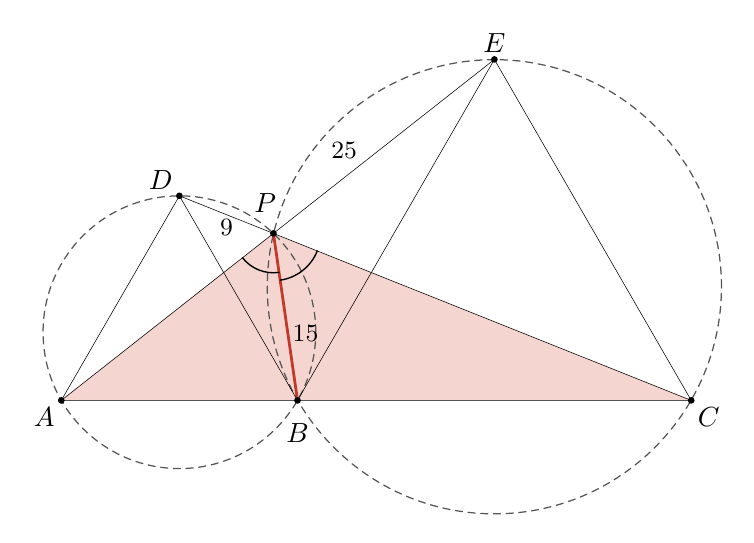
\begin{tikzpicture}
\tkzDefPoint(0.0,0.0){A} %! A = (0, 0)
\tkzDefPoint(3.0000000,0.0){B} %! B = (21, 0)
\tkzDefPoint(8.0000000,0.0){C} %! C = (56, 0)
\tkzDefPoint(1.5000000,2.5980762){D} %! D = (21/2, 21*sqrt(3)/2)
\tkzDefPoint(5.5000000,4.3301270){E} %! E = (77/2, 35*sqrt(3)/2)
\tkzDefPoint(2.6938776,2.1208785){P} %! P = (132/7, 60*sqrt(3)/7)
\tkzDefPoint(1.5000000,0.86602540){Oa} %! Oa = (21/2, 7*sqrt(3)/2)
\tkzDefPoint(5.5000000,1.4433757){Ob} %! Ob = (77/2, 35*sqrt(3)/6)
%! fact on_segment(B, A, C)
%! fact on_segment(P, A, E)
%! fact on_segment(P, C, D)
%! fact equal(dist(A, B), dist(B, D))
%! fact equal(dist(A, B), dist(A, D))
%! fact equal(dist(B, C), dist(C, E))
%! fact equal(dist(B, C), dist(B, E))
%! fact concyclic(A, B, P, D)
%! fact concyclic(B, C, E, P)
%! fact on_circle(P, Oa, dist(Oa, A))
%! fact on_circle(P, Ob, dist(Ob, B))
%! fact dist(P, D) == 9
%! fact dist(P, E) == 25
%! fact dist(P, A) == 24
%! fact dist(P, C) == 40
%! fact dist(P, B) == 15
%! fact dist(A, C) == 56
%! fact angle(A, P, B) == 60
%! fact angle(B, P, C) == 60
%! fact dist(P, D) == dist(P, A) - dist(P, B)
%! fact dist(P, E) == dist(P, C) - dist(P, B)
\tkzFillPolygon[color=figaccenttint](A,P,C)
\tkzDrawCircle[aux](Oa,A)
\tkzDrawCircle[aux](Ob,B)
\tkzDrawPolygon(A,B,D)
\tkzDrawPolygon(B,C,E)
\tkzDrawSegments(A,E C,D)
\tkzDrawSegment[key](P,B)
\tkzMarkAngle[size=.5,arc=l,mark=none,mk](A,P,B)
\tkzMarkAngle[size=.6,arc=l,mark=none,mk](B,P,C)
\tkzDrawPoints(A,B,C,D,E,P)
\tkzLabelPoint[below left,lbl](A){$A$}
\tkzLabelPoint[below=6pt,lbl](B){$B$}
\tkzLabelPoint[below right,lbl](C){$C$}
\tkzLabelPoint[above left,lbl](D){$D$}
\tkzLabelPoint[above,lbl](E){$E$}
\tkzLabelPoint[above=5pt,xshift=-3pt,lbl](P){$P$}
\tkzLabelSegment[below,pos=.5,len](P,D){$9$}
\tkzLabelSegment[above left,pos=.4,len](P,E){$25$}
\tkzLabelSegment[right,pos=.6,len](P,B){$15$}
\end{tikzpicture}
\end{document}
